\chapter{Estado del Arte}

\section{Estimación de la edad}
% La estimación de la edad, al ser un componente sumamente importante a la hora de obtener el PB, ha tomado mayor interés de los investigadores a comienzos del siglo actual y teniendo una tendencia creciente en el número de publicaciones. Puede observarse en la Figura \ref{fig:scopusData} la cantidad de publicaciones existentes en la base de datos \textit{Scopus} que hacen referencia tanto a AF como a la estimación de edad\footnote{Consulta realizada: \code{(TITLE-ABS-KEY (forensic AND anthropology AND age AND estimation))}.}, desde 1977 se tienen 1419 publicaciones registradas. 

% Por otro lado, y afirmando lo mencionado sobre la precariedad tecnológica que posee esta área de conocimiento, existe un número muy limitado de publicaciones que hagan alguna mención no solamente de DL o ML sino de técnicas de IA en general\footnote{Consulta realizada: \code{(TITLE-ABS-KEY (((deep AND learning) OR (machine AND learning) OR (soft AND computing) OR (artificial AND intelligence) OR (data AND mining)) AND forensic AND anthropology AND age AND estimation))}.}, es decir, que incluso relajando los términos de búsqueda para englobar toda el área de IA, se tienen solamente 30 publicaciones que han surgido mayoritariamente a mediados de la década pasada. Finalmente, solo hay cinco artículos que combinan IA con modelos tridimensionales para la estimación de edad por medio de AF\footnote{Consulta realizada: \code{(TITLE-ABS-KEY ( ((deep AND learning) OR (machine AND learning) OR (soft AND computing) OR (artificial intelligence) OR (data AND mining) ) AND forensic AND anthropology AND age AND estimation AND 3d))}.}. Esto se interpreta como un indicador de lo novedoso y pionero de este trabajo.

La estimación de la edad, al ser un componente clave en la determinación del PB, ha captado un creciente interés por parte de la comunidad científica desde comienzos del presente siglo, evidenciando una tendencia al alza en el número de publicaciones. En la Figura \ref{fig:scopusData} se muestra la evolución del volumen de publicaciones indexadas en la base de datos \textit{Scopus} que hacen referencia tanto a la AF como a la estimación de edad por medio de la cadena de búsqueda \ref{code__scopus_af}, registrándose un total de 1419 trabajos desde el año 1977.

Sin embargo, y en línea con lo ya mencionado respecto a la limitada sofisticación tecnológica de esta disciplina, el número de publicaciones que integran técnicas de IA es considerablemente más reducido, al realizarse la consulta con la cadena \ref{code__scopus_af_ai} se identifican 71 artículos.

Finalmente, al acotar aún más la búsqueda a estudios que combinen IA con modelos tridimensionales para la estimación de edad mediante AF con la cadena \ref{code__scopus_af_ai_3d}, se obtienen únicamente ocho artículos. Esta escasa representación refuerza el carácter novedoso y pionero del presente trabajo.

\begin{lstlisting}[caption={Cadena de búsqueda de \textit{Scopus} para obtener publicaciones de AF que referencian la estimación de la edad.}, captionpos=b, label=code__scopus_af, style=Consola]
(TITLE-ABS-KEY (forensic AND anthropology AND age AND estimation))
\end{lstlisting}
            
\begin{lstlisting}[caption={Cadena de búsqueda de \textit{Scopus} para obtener publicaciones de AF que referencian la estimación de la edad y hacen uso de alguna técnica de IA}, captionpos=b, label=code__scopus_af_ai, style=Consola]
(TITLE-ABS-KEY (((deep AND learning) OR (machine AND learning) OR (soft AND computing) OR (artificial AND intelligence) OR (data AND mining)) AND forensic AND anthropology AND age AND estimation))
\end{lstlisting}
            
\begin{lstlisting}[caption={Cadena de búsqueda de \textit{Scopus} para obtener publicaciones de AF que referencian la estimación de la edad, hacen uso de alguna técnica de IA y utilizan datos 3D.}, captionpos=b, label=code__scopus_af_ai_3d, style=Consola]
(TITLE-ABS-KEY ( ((deep AND learning) OR (machine AND learning) OR (soft AND computing) OR (artificial AND intelligence) OR (data AND mining) ) AND forensic AND anthropology AND age AND estimation AND 3d))
\end{lstlisting}

\begin{figure}[h]
    \centering
    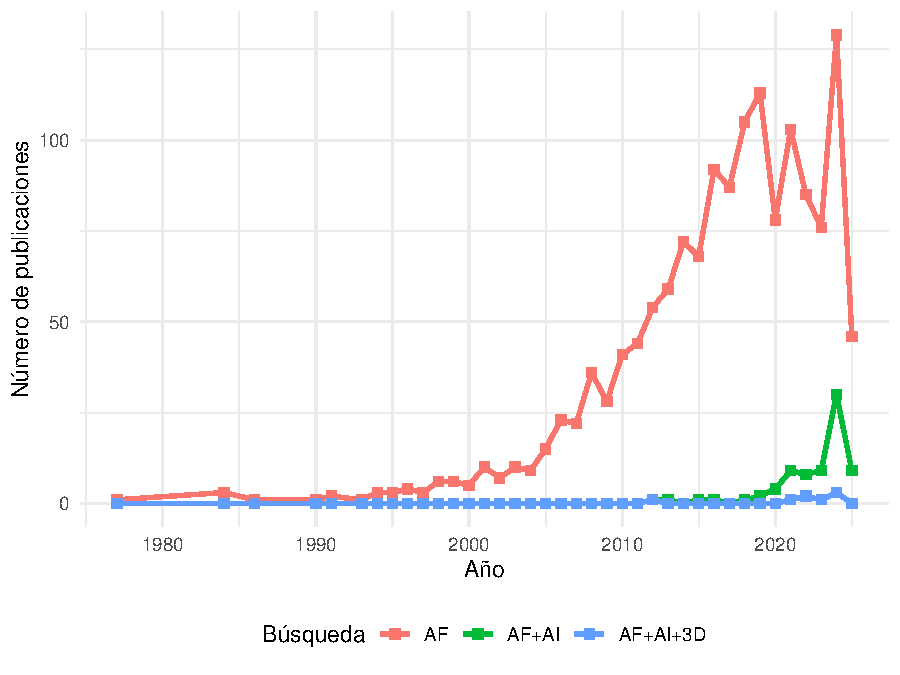
\includegraphics[width=\linewidth]{figures/3_sota/scopus_pubs.pdf}
    \caption[Publicaciones por año de AF, AF+IA y AF+IA+3D en Scopus]{Número de publicaciones en \textit{Scopus} en función del año a fecha de 08/04/2025. En {\color{Red} \textbf{rojo}} se muestran las publicaciones que mencionan AF y la estimación de la edad (1419 publicaciones), en {\color{LimeGreen} \textbf{verde}} aquellas que adicionalmente mencionan alguna técnica de IA (71 publicaciones) y en {\color{Blue} \textbf{azul}} aquellas que también mencionan el uso de 3D (8 publicaciones).}
    \label{fig:scopusData}
\end{figure}

A continuación se presenta el estado del arte de tanto en los métodos tradicionales utilizando la sínfisis del pubis y, brevemente, aquellos utilizados en otras estructuras óseas. Luego se presentan los métodos de estimación automáticos centrándose en la sínfisis del pubis con el uso de DL y modelos 3D.

\subsection{Métodos tradicionales para restos óseos}

En cuanto al cráneo, los métodos más comúnmente empleados para la estimación de la edad son los propuestos por Meindl y Lovejoy \cite{meindl1985ectocranial}, Acsádi y Nemeskéri \cite{acsadi1970history}, y Mann \cite{mann1991maxillary}. Estos enfoques se basan en el análisis del grado de osificación de las articulaciones fibrosas que conectan los distintos huesos del cráneo, conocidas como suturas craneales. De acuerdo con una revisión reciente \cite{ruengdit2020cranial}, estos métodos tienden a producir resultados erráticos y con baja precisión. Por ello, se recomienda su utilización únicamente como complemento de otros métodos basados en diferentes estructuras óseas. No obstante, el mismo estudio señala que la incorporación de nuevas tecnologías, como la tomografía axial computarizada, ha contribuido a reducir los márgenes de error en la estimación de edad, como se evidencia en trabajos como \cite{chiba2013age, boyd2015use}.

Respecto a las costillas, el método más utilizado es el desarrollado por İșcan y Loth \cite{icscan1984age, icscan1985age}, que se enfoca en los cambios morfológicos del extremo ventral de la cuarta costilla asociados al envejecimiento. Sin embargo, este método presenta diversas limitaciones, tales como sesgos poblacionales, escasa reproducibilidad entre distintas poblaciones y errores tanto intraevaluador como interevaluador de magnitud moderada \cite{fanton2010critical, hartnett2010analysis}. Actualmente, el método ha comenzado a incorporar de forma limitada técnicas de imagen como la tomografía axial computarizada para mejorar su precisión \cite{blaszkowska2019validation}.

En cuanto a la cara auricular del ilion, los métodos más utilizados para la estimación de la edad son los propuestos por Lovejoy \cite{lovejoy1985chronological} y por Buckberry y Chamberlain \cite{buckberry_age_2002}. Al igual que otros métodos tradicionales, estos también presentan limitaciones importantes en cuanto a la precisión de las estimaciones y están sujetos a diversos sesgos poblacionales \cite{falys2006auricular, michopoulou2017auricular}. En la actualidad, se ha intentado mejorar la fiabilidad de estos métodos mediante la incorporación de técnicas de imagen como la tomografía axial computarizada \cite{villa2013reliability, barrier2009age}, así como mediante la aplicación de enfoques analíticos basados en estadística bayesiana. No obstante, los resultados obtenidos con estos métodos complementarios han sido mixtos y no concluyentes \cite{nikita2018evaluation}.

\subsection{Métodos tradicionales utilizando la sínfisis del pubis}

La sínfisis del pubis constituye el hueso más comúnmente empleado en la estimación de la edad en contextos forenses, como se mencionó previamente en la Sección \ref{daIntro_ProblemDef}. En la actualidad, el método más difundido para este propósito es el propuesto por Suchey-Brooks \cite{RefWorks:RefID:20-brooks1990skeletal}, una variante modernizada del método original desarrollado por Todd. Ambos métodos se basan en la observación de características morfológicas específicas de la superficie de la sínfisis púbica (véase Tabla \ref{table:themBones}) para clasificar el hueso dentro de un determinado rango etario. El método de Todd establece una clasificación en 10 fases o intervalos de edad, mientras que el método de Suchey-Brooks reduce esta categorización a 6 fases, aunque estas presentan un mayor grado de solapamiento entre sí. Los rangos definidos por ambos métodos pueden consultarse en las Tablas \ref{table:age_todd_} y \ref{table:age_suchey_brooks}.

\begin{table}[h]
\centering
\begin{tabular}{|c|c|}
\hline
\rowcolor[HTML]{FFCB2F} 
{Etapa} & {Rango de Edad} \\ \hline
I & 18-19 \\ \hline
II & 20-21 \\ \hline
III & 22-24 \\ \hline
IV & 25-26 \\ \hline
V & 27-30 \\ \hline
VI & 30-35 \\ \hline
VII & 35-39 \\ \hline
VIII & 39-44 \\ \hline
IX & 45-50 \\ \hline
X & 50+ \\ \hline
\end{tabular}
\caption{Rangos de edad del Método de Todd}
\label{table:age_todd_}
\end{table}

\begin{table}[h]
\centering
\begin{tabular}{|c|c|}
\hline
\rowcolor[HTML]{FFCB2F} 
{Etapa} & {Rango de Edad} \\ \hline
I & 15-23 \\ \hline
II & 19-34 \\ \hline
III & 21-46 \\ \hline
IV & 23-57 \\ \hline
V & 27-66 \\ \hline
VI & 34-86 \\ \hline
\end{tabular}
\caption{Rangos de edad del Método de Suchey-Brooks}
\label{table:age_suchey_brooks}
\end{table}

Según un metaanálisis reciente \cite{schanandore2022accuracy}, el método de Suchey-Brooks se posiciona como uno de los más precisos para la estimación de la edad en contextos forenses. No obstante, diversos autores recomiendan su aplicación con precaución debido a sus limitaciones inherentes \cite{priya2017methods}. En la actualidad, el uso de imágenes provenientes de tomografías computarizadas permite aplicar el método directamente sobre modelos volumétricos, replicando de manera virtual el análisis que tradicionalmente se realiza sobre el hueso físico. Algunos estudios \cite{wade2011preliminary,villa2013forensic,lottering2014morphometric,lopez2015image} han aprovechado esta tecnología para observar los cambios en la densidad ósea interna que ocurren con el envejecimiento, con el fin de refinar los procesos de estimación. Sin embargo, a pesar de la incorporación puntual de estas tecnologías, el método continúa dependiendo de características morfológicas subjetivas. Esta subjetividad conduce a que las estimaciones finales estén fuertemente influenciadas por la experiencia del perito, más que por una evaluación objetiva y sistemática de los datos, lo cual compromete tanto la efectividad como la credibilidad del proceso de estimación \cite{garvin_current_2012}.

\subsection{Métodos automáticos utilizando la sínfisis del pubis}

Los primeros intentos por reemplazar los métodos subjetivos en la estimación de edad a partir de la sínfisis del pubis surgen a inicios de la década de 2010 con el estudio realizado por Biwasaka et al. \cite{biwasaka2013three}. En dicho trabajo se calcula analíticamente la curvatura media de la superficie de la sínfisis del pubis, obtenida mediante escaneo 3D, para evaluar el grado de concavidad o convexidad del hueso en relación con los intervalos de edad definidos por el método de Suchey-Brooks. Aunque se utilizó una muestra de 145 huesos y se concluye que existe una relación entre las fases del método y la curvatura, el estudio no reporta métricas estadísticas cuantitativas que respalden los hallazgos.

Villa et al. \cite{villa2015quantitative} amplían el enfoque anterior al definir cinco variables derivadas del análisis de curvatura: la media del valor absoluto de la curvatura, el 10\% de curvaturas más altas, el 10\% más bajas, el porcentaje de superficie con curvaturas mayores que cero (regiones convexas) y el porcentaje con curvaturas entre $-0.01$ y $0.01$ (regiones planas). Se emplearon dos conjuntos de datos: uno con 24 huesos, que arrojó una correlación de Spearman moderada a fuerte ($\rho=0.60-0.93$), y otro con 98 huesos, con correlaciones más débiles ($\rho=0.29-0.51$), comparables a los valores alcanzados por métodos manuales, lo cual demuestra el potencial de este enfoque.

En Slice y Algee-Hewitt \cite{slice2015modeling} se introdujo una métrica denominada \textit{Slice Algee-Hewitt Score} (SAH-Score), basada en un análisis de componentes principales (PCA) aplicado a los vértices de mallas 3D de la sínfisis del pubis. Esta métrica cuantifica la complejidad superficial del hueso y se utiliza como predictor en un modelo de regresión lineal para estimar la edad. Con una muestra de 41 huesos, se obtuvo un error cuadrático medio (RMSE) de 17.15 años, con predicciones que coinciden razonablemente con los intervalos del método de Suchey-Brooks.

Stoyanova et al. \cite{stoyanova2015enhanced} emplean el algoritmo \textit{Thin Plate Splines} (TPS) para estimar la energía de flexión (\textit{bending energy}, BE) requerida para transformar una superficie plana en la forma tridimensional del hueso. Esta métrica se usa en un modelo de regresión lineal entrenado con 44 mallas, obteniendo un RMSE de 19 años. En un trabajo posterior \cite{stoyanova2017computational}, los autores combinan múltiples características (SAH-Score, BE y curvatura del borde ventral) para entrenar un modelo de regresión multivariable con 93 muestras, logrando un RMSE entre 13.7 y 16.5 años.

Villar et al. \cite{villar2017first} utilizan Árboles de Decisión Difusos (\textit{Fuzzy Decision Trees}, FDT) para generar reglas que permitan clasificar los huesos en los intervalos de edad del método de Todd, usando 74 muestras etiquetadas por dos expertos. El modelo alcanza un error absoluto medio (MAE) de 1.68 años respecto al intervalo correspondiente, aunque el número reducido de muestras impidió cubrir todos los rangos etarios.

En Gámez-Granados et al. \cite{granados} se propone un sistema explicable basado en reglas utilizando el clasificador ordinal NSLVOrd \cite{gamez2016ordinal}, el cual clasifica 892 muestras de sínfisis del pubis dentro de los 10 intervalos definidos por Todd, utilizando las nueve características tradicionales etiquetadas por expertos. Aunque el enfoque es de clasificación, puede adaptarse para predecir directamente la edad. El modelo reporta un RMSE de 12.34 años y un MAE de 10.38 años.

Kotěrová et al. \cite{kotverova2018age} exploran nueve métodos de regresión aplicados a características extraídas manualmente por expertos. Con una muestra de 941 huesos, la regresión lineal múltiple ofrece el mejor desempeño, con un RMSE de 12.1 años y un MAE de 9.7 años. En una extensión del estudio \cite{koterova_computational_2022}, se incorporan mallas 3D y se introducen dos nuevos enfoques: uno que caracteriza la superficie del hueso mediante la energía de Dirichlet, y otro basado en una CNN entrenada con múltiples proyecciones 2D del modelo 3D. Los mejores resultados obtenidos son un MAE de 11.7 y 10.6 años, respectivamente.

Por último, Bermejo et al. \cite{bermejo_interpretable_2025} proponen un método semi-automático e interpretable, basado en regresión simbólica obtenida mediante Programación Genética, utilizando como entrada las nueve características del método de Todd. El mejor modelo generado reporta un MSE de 10.81 años y un MAE de 8.55 años. Aunque estos resultados representan una mejora frente al método propuesto por Kotěrová, los autores consideran ambos enfoques como equivalentes y complementarios, dado que el modelo de Bermejo requiere el etiquetado experto de las características, mientras que el de Kotěrová es completamente automático.

Los tres últimos estudios mencionados son los más cercanos al enfoque de este TFM. En \cite{koterova_computational_2022} se emplea una CNN para extraer automáticamente características de la sínfisis del pubis a partir de un modelo 3D, aunque con el objetivo de estimar directamente la edad, a diferencia del presente proyecto, cuyo objetivo es clasificar el hueso según las características del método de Todd. En esta línea, los trabajos de \cite{villar2017first} y \cite{bermejo_interpretable_2025} sí hacen uso explícito de dichas características, pero partiendo de información etiquetada por expertos. Ambos enfoques permiten obtener reglas explicables para clasificar un hueso dentro de los intervalos de edad, o bien estimar un valor numérico de edad, pero no permiten identificar directamente las características morfológicas en la sínfisis del pubis. En este sentido, el presente trabajo se plantea como pionero, ya que, según la literatura consultada, no existe otro estudio que utilice técnicas de DL para extraer automáticamente las características de Todd a partir de modelos 3D.

\section{Representaciones 3D en \textit{Deep Learning}}
Como se discutió en la Sección \ref{3d_reps}, existen múltiples formas de representar datos tridimensionales para su utilización en técnicas de DL. En esta sección se analiza cuál de estas representaciones resulta más adecuada para la extracción automática de características morfológicas orientadas a la estimación de la edad, y se presentan los avances más recientes asociados a dicha representación.

La representación mediante nubes de puntos es la más sencilla, ya que consiste únicamente en un conjunto de coordenadas tridimensionales. Sin embargo, esta simplicidad implica que conceptos clave como la vecindad local y la conectividad entre puntos no están bien definidos. Esto dificulta la aplicación directa de operaciones típicas de CNNs, generando ambigüedades que afectan negativamente el rendimiento del modelo, especialmente en escenarios que requieren un alto nivel de detalle. Por estas razones, esta representación se descarta para este trabajo.

La representación RGB-D, aunque útil para algunas aplicaciones, es esencialmente una representación 2.5D y, por lo tanto, no tiene la capacidad de capturar completamente la complejidad de la geometría tridimensional. Dado que el objetivo es analizar en detalle la morfología ósea, esta representación también se descarta.

Las proyecciones y vistas múltiples permiten aprovechar arquitecturas clásicas de CNNs mediante la conversión del objeto 3D en una o varias imágenes 2D. Sin embargo, este enfoque conlleva pérdida de información topológica al realizar la proyección, y puede presentar problemas en superficies complejas donde partes del modelo ocluyen otras, generando aún más pérdida de información. Por ello, ambas representaciones se descartan igualmente.

Los descriptores 3D simplifican un modelo tridimensional en una representación compacta o \say{firma}, que resulta útil para tareas de reconocimiento global. Sin embargo, dado que este trabajo se enfoca en analizar detalladamente la topología de la superficie ósea, esta simplificación resulta inadecuada. Además, los descriptores son más eficaces en tareas de aprendizaje no supervisado que en supervisado, lo cual refuerza su exclusión. Por motivos similares, las representaciones basadas en grafos también se descartan, ya que requieren una transformación intermedia del modelo 3D que complica el tratamiento directo de su geometría.

Las representaciones volumétricas, como los vóxeles, permiten describir el volumen completo del objeto en una rejilla tridimensional. Sin embargo, esta aproximación tiene un elevado coste computacional debido a la necesidad de realizar operaciones sobre espacios vacíos, lo que incrementa significativamente el uso de memoria. Además, este tipo de representación no permite capturar con suficiente precisión los detalles finos de la superficie, lo que la hace inadecuada para el problema planteado.

La representación seleccionada en este trabajo es la de mallas poligonales tridimensionales. Estas son ampliamente utilizadas en el ámbito de la informática gráfica, lo que ha dado lugar a una gran variedad de herramientas y algoritmos para su procesamiento y análisis. Además, la mayoría de escáneres 3D empleados en AF generan directamente este tipo de representación, lo que facilita el flujo de trabajo. Las mallas son una representación eficiente y precisa: en zonas lisas y planas se utilizan pocos polígonos, mientras que en zonas con geometría compleja la densidad de polígonos aumenta, permitiendo capturar detalles intrincados. Desde el punto de vista del procesamiento mediante CNNs, las mallas ofrecen una ventaja adicional, ya que proporcionan información explícita sobre la conectividad entre vértices, lo que permite definir vecindarios locales de forma natural y estructurada.

\subsection{Mallas poligonales}

En el trabajo pionero de Feng et al. \cite{feng2019meshnet} se propone MeshNet, el primer \textit{framework} basado en CNNs diseñado para procesar directamente mallas 3D. En este enfoque, la unidad básica de procesamiento no son los vértices ni los vóxeles, sino las caras triangulares de la malla, las cuales permiten mantener la conectividad topológica y facilitan la definición de operaciones análogas a las convoluciones en imágenes, donde los píxeles tienen vecindarios bien definidos.

Cada cara triangular es descrita por dos tipos de características, que funcionan como el análogo del valor RGB en imágenes: características espaciales y características estructurales.
\begin{itemize}
    \item Las características espaciales se calculan a partir de la posición del centroide de cada triángulo, representando su ubicación en el espacio.
    \item Las características estructurales se dividen en dos componentes: una que captura la estructura interna de la cara (por ejemplo, ángulos internos o proporciones entre lados), y otra que captura la estructura externa, que examina el vecindario local de cada cara, permitiendo aprender sobre la disposición relativa entre caras adyacentes.
\end{itemize}
Además, se redefine la operación de convolución para que trabaje de forma coherente con estas representaciones. El bloque convolucional propuesto consta de dos partes:

\begin{itemize}
    \item Una combinación de características espaciales y estructurales, que permite mezclar la posición con la forma local del triángulo.
    \item Una agregación estructural, que aprende a fusionar la información del vecindario de caras.
\end{itemize}
Ambas operaciones generan nuevas representaciones que se pasan al siguiente bloque de la red, permitiendo una jerarquía de aprendizaje similar a las CNNs tradicionales.

Para la validación del modelo, se utilizó el conjunto de datos ModelNet40 \cite{wu20153d}, una base de datos ampliamente utilizada en tareas de clasificación de objetos 3D. MeshNet alcanzó un 91.9\% de precisión en la tarea de clasificación, superando a modelos basados en nubes de puntos, representaciones volumétricas y métodos basados en múltiples vistas.

En Hanocka et al. \cite{hanocka2019meshcnn} se propone otro \textit{framework} denominado MeshCNN, publicado casi en paralelo con MeshNet, con solo unos meses de diferencia. A diferencia de MeshNet, que toma como unidad básica de procesamiento las caras triangulares, MeshCNN utiliza las aristas que conectan los vértices de la malla como unidad convolucional, lo que constituye el análogo al píxel en una imagen. En lugar de describir las caras con múltiples tipos de descriptores, cada arista es caracterizada mediante un vector de cinco componentes, compuesto por atributos geométricos específicos de la arista que son invariantes a traslación y rotación. Esto permite realizar operaciones de convolución de manera más directa y robusta frente a transformaciones espaciales. Una de las contribuciones más importantes de MeshCNN es la implementación de una operación de \textit{pooling} adaptativo, donde la red aprende automáticamente qué regiones de la malla puede simplificar y cuáles debe preservar, optimizando así la tarea de aprendizaje.

Los experimentos se realizaron en distintos conjuntos de datos, obteniendo un 98.6\% de exactitud en SHREC30 \cite{lian2011shape} y un 92.16\% en un conjunto de cubos esculpidos con diferentes formas \cite{latecki2000shape}.

En Schneider et al. \cite{schneider_medmeshcnn_2021} se introduce MedMeshCN como una extensión de MeshCNN enfocada en reducir el elevado consumo de memoria de la implementación original. Esta optimización se logra mediante modificaciones en la operación de \textit{pooling}, con énfasis en aplicaciones médicas, particularmente en tareas de segmentación de mallas 3D. Para su validación, se utilizaron 94 mallas de aneurismas intracraneales: 65 provenientes del conjunto de datos AneuRisk65 \cite{sangalli2014aneurisk65} y el resto provistas por el Hospital Universitario de Magdeburgo, Alemania. Se reporta un índice de Jaccard promedio de 63.24\% en todas las clases, con un 71.4\% específicamente para la segmentación de aneurismas, concluyéndose que el \textit{framework} tiene potencial para aplicaciones en el ámbito médico.

De forma pararela en \cite{mandado_surface_2021}, se presenta MeshCNN+, otra variante cuyo objetivo es también mitigar el alto uso de memoria de MeshCNN, mediante una nueva implementación del \textit{pooling} y la posibilidad de entrenamiento distribuido en múltiples máquinas. Este estudio también se centra en tareas de segmentación y utiliza el conjunto de datos ABC \cite{Koch_2019_CVPR}, que contiene más de un millón de mallas generadas mediante software de diseño asistido por computadora (CAD). El modelo alcanzó una exactitud del 86.2\%, aunque se observó que tenía dificultades para segmentar clases poco representadas en la superficie de las mallas.

Por último, Kim y Chae \cite{kim_exmeshcnn_2022} introducen ExMeshCNN, una expansión y, al mismo tiempo, una mezcla entre las propuestas de MeshNet y MeshCNN, ya que combina la extracción de características tanto de las caras triangulares como de las aristas. Para ello, la capa inicial de cualquier modelo basado en esta técnica incorpora dos extractores de características geométricas y geodésicas a partir de las caras triangulares. Estos extractores, denominados descriptores, actúan como filtros de convolución 1D con parámetros entrenables. Las capas posteriores aplican convoluciones 1D sobre las caras triangulares y sus vecindades locales.

A diferencia de MeshCNN, que emplea operaciones de \textit{pooling} para aportar explicabilidad al modelo, ExMeshCNN permite aplicar técnicas como Grad-CAM gracias al uso de convoluciones 1D, lo que posibilita identificar directamente qué caras tienen mayor relevancia en la generación de una salida específica.

En los experimentos realizados con los conjuntos de datos ModelNet40 y Manifold40, ExMeshCNN alcanzó los mejores resultados reportados hasta la fecha, con 93\% y 93.4\% de \textit{accuracy} respectivamente, superando a modelos como MeshCNN y MeshNet++. De igual forma, en los conjuntos SHREC11 y el de cubos esculpidos, alcanzó un \textit{accuracy} del 100\%, posicionándose así como el \textit{framework} actual de referencia en el uso de \textit{Deep Learning} sobre mallas 3D.